\documentclass[12pt, a4paper, oneside]{ctexart}
\usepackage{amsmath, amsthm, amssymb, appendix, bm, graphicx, hyperref, mathrsfs}
\usepackage{float}
\usepackage{booktabs} 
\usepackage{caption}
\usepackage{geometry}
\geometry{margin=1in}

\title{\textbf{判别分析}}
\author{王一鑫}
\date{\today}
\linespread{1.5}
\newtheorem{theorem}{定理}[section]
\newtheorem{definition}[theorem]{定义}
\newtheorem{lemma}[theorem]{引理}
\newtheorem{corollary}[theorem]{推论}
\newtheorem{example}[theorem]{例}
\newtheorem{proposition}[theorem]{命题}
\renewcommand{\abstractname}{\Large\textbf{摘要}}
\usepackage{listings}
\usepackage{xcolor}
\definecolor{mygreen}{rgb}{0,0.6,0}
\definecolor{mygray}{rgb}{0.5,0.5,0.5}
\definecolor{mymauve}{rgb}{0.58,0,0.82}


\lstset{numbers=left, %设置行号位置
	numberstyle=\tiny\color{mygray}, %设置行号大小
	basicstyle=\footnotesize,
	keywordstyle=\color{blue}, %设置关键字颜色
	commentstyle=\color{mygreen}, %设置注释颜色
	frame=single, %设置边框格式
	rulecolor=\color{black},
	escapeinside=``, %逃逸字符(1左面的键),用于显示中文
	%breaklines, %自动折行
	extendedchars=false, %解决代码跨页时,章节标题,页眉等汉字不显示的问题
	xleftmargin=2em,xrightmargin=2em, aboveskip=1em, %设置边距
	tabsize=2, %设置tab空格数
	showspaces=false,%不显示空格
	breaklines=true,  
	stringstyle=\color{orange}
}


\begin{document}
	
	\maketitle
	
	\setcounter{page}{0}
	\maketitle
	\thispagestyle{empty}
	
	\begin{abstract} 
		判别分析作为多元统计分析的重要分支,在分类与识别问题中具有广泛应用. 本文系统介绍了三类经典判别方法:\textbf{距离判别}、\textbf{Bayes判别}和\textbf{Fisher判别},并详细推导了其判别函数的数学原理和判别准则;通过对经典数据集如三文鱼数据和鸢尾花数据的实证分析,展示了判别函数的建构过程与判别效果,并与支持向量机(SVM)进行了对比研究. SVM部分介绍了线性核、多项式核和径向基核的判别思想与模型实现,并在心脏病预测数据上进行了性能评估. 结果表明,传统判别方法在模型可解释性方面具有优势,而SVM在复杂数据结构下具有更强的分类能力. 本文为判别方法的学习和实用提供了理论基础与算法实现参考.
		
		\par\textbf{关键词:}判别分析;Bayes判别;Fisher判别;支持向量机
	\end{abstract}
	
	
	\newpage
	\pagenumbering{Roman}
	\setcounter{page}{1}
	\tableofcontents
	\newpage
	\setcounter{page}{1}
	\pagenumbering{arabic}
	
	\section{判别分析}
	
	\subsection{问题背景}
	
	判别分析(discriminant analysis)属于监督学习(supervised learning)方法,使用具有类别信息的观测数据建立一个分类器(classifier)或者分类法则(classification rule),对新的数据可以利用分类规则判断新数据观测的类别. 训练样本中既有用来分类的解释变量(自变量),又有真实的类别(标签,因变量).
	
	在生产、科研和日常生活中经常遇到如何根据观测到的数据资料对所研究的对象进行判别归类的问题. 例如在医学诊断中,一个患者肺部有阴影,医生要判断患者是肺结核、肺部良性肿瘤还是肺癌. 这里肺结核患者、肺部良性肿瘤患者、肺癌患者组成三个总体,患者来源于这三个总体之一,判别分析的目的是通过测得患者的指标(阴影的大小、边缘是否光滑、体温多少等)来判断患者应该属于哪个总体(即判断患者生什么病).
	
	常用判别分析方法有距离判别、Fisher 判别和 Bayes 判别,支持向量机(SVM, Support Vector Machine)也是判别式分类方法的一种.
	
	当标签(因变量)只有两个类时,判别分析问题与假设检验问题有相似之处. 假设检验问题更强调拒绝零假设的结论一定要可靠,所以更重视对立假设;两类的判别问题并不强调某个类别,或者按照先验概率、损失函数对不同类别施加不同的影响.
	
	\subsection{距离判别}
	\subsubsection{模型原理}
	距离判别的思想是计算每个样品与各类中心的距离,把样品分到最近的一类. 常用距离为欧式距离与马氏(Mahalonobis)距离.
	\begin{definition}
		设 $X = (X_1, X_2, \ldots, X_p)^T$ 与 $Y = (Y_1, Y_2, \ldots, Y_p)^T$ 是两个随机向量,有相同的协方差矩阵 $\Sigma$,定义 $X$ 的观测值 $x = (x_1, x_2, \ldots, x_p)^T$ 与 $Y$ 的观测值 $y = (y_1, y_2, \ldots, y_p)^T$ 的马氏距离为
		\begin{equation}
			d(x, y) = \sqrt{(x - y)^T \Sigma^{-1} (x - y)}. \label{Maha}
		\end{equation}
	\end{definition}
	
	设有两个总体 $G_1, G_2$,均值分别为 $\mu_1, \mu_2$,$\mu_1 \ne \mu_2$. 有共同的协方差矩阵 $\Sigma$。在 $\mu_1, \mu_2, \Sigma$ 已知时,为了判断一个样品 $x$ 属于哪一个总体(类),可以用如下判别规则:
	\[
	\left\{
	\begin{aligned}
		&\text{判} x \in G_1,\quad d(x, \mu_1) \leq d(x, \mu_2), \\
		&\text{判} x \in G_2,\quad d(x, \mu_1) > d(x, \mu_2).
	\end{aligned}
	\right.
	\]
	
	为判断上述条件,只要计算 $d^2(x, \mu_2) - d^2(x, \mu_1)$ 的正负号,非负时判入 $G_1$,负号时判入 $G_2$.
	
	计算距离平方的差为
	\begin{equation}
		d^2(x, \mu_2) - d^2(x, \mu_1) = 2(\mu_1 - \mu_2)^T \Sigma^{-1} \left(x - \frac{\mu_1 + \mu_2}{2}\right) \label{dsquareminus}
	\end{equation}

	\begin{definition}
		令 $a = \Sigma^{-1} (\mu_1 - \mu_2)$,则$x$ 的线性判别函数为
		\begin{align}
			W(x) \triangleq \frac{1}{2} \left(d^2(x, \mu_2) - d^2(x, \mu_1)\right)
			= a^T \left(x - \frac{\mu_1 + \mu_2}{2} \right)\label{LDF}
		\end{align}
		其中$a$ 为判别系数. 
		
	\end{definition}
	此时对应的判别规则为:
	\[
	\left\{
	\begin{aligned}
		&\text{判} x \in G_1,\quad \text{当 } W(x) \geq 0, \\
		&\text{判} x \in G_2,\quad \text{当 } W(x) < 0.
	\end{aligned}
	\right.
	\]
	\subsubsection{代码实践}
	\begin{example}
		某种昆虫的体长与翅长用来判别性别. 雌虫(总体 $G_1$)平均值 $\mu_1 = (6, 5)^T$,雄虫(总体 $G_2$)平均值 $\mu_2 = (8, 6)^T$,雄虫体型较大. 两个总体共同的协方差矩阵为
		\[
		\Sigma = \begin{pmatrix}
			9 & 2 \\
			2 & 4
		\end{pmatrix}。
		\]
		
		现有某虫测量值为 $x_{1} = (7.2, 5.6)^T$,$x_{2} = (6.3, 4.9)^{T}$,用距离判别法做判别,判断其性别. 用 R 程序实现.
	\end{example}
	首先定义线性判别函数:
	\begin{lstlisting}[language=R]
		# 定义线性判别函数
		W <- function(x, mu1, mu2, Sigma) {
			a <- solve(Sigma, mu1 - mu2) 
			mu3 <- (mu1 + mu2) / 2 
			sum(a * (x - mu3)) 
		}
	\end{lstlisting}
	用线性判别法建立雌虫与雄虫的判别公式,只需要输入两个中心,与共同的协方差阵:
	\begin{lstlisting}[language=R]
		# 设置组均值和协方差矩阵
		mu1 <- c(6, 5) # 雌虫平均值
		mu2 <- c(8, 6) # 雄虫平均值
		Sigma <- rbind(c(9, 2), c(2, 4)) # 协方差矩阵
	\end{lstlisting}
	对两个测量值做判别:
	\begin{lstlisting}[language=R]
		x1 <- c(7.2, 5.6)
		y1 <- W(x1, mu1, mu2, Sigma)
		x2 <- c(6.3, 4.9)
		y2 <- W(x2, mu1, mu2, Sigma)
	\end{lstlisting}
	当测量值为$x_{1} = (7.2, 5.6)^T$时,线性判别函数数值为$-0.053125$判入第二类,雄虫;
	当测量值为$x_{2} = (6.3, 4.9)^{T}$时,线性判别函数数值$0.225$判入第一类,雌虫.
	
	\subsection{Bayes判别}
	\subsubsection{判别准则}
	距离判别不考虑某一总体实际出现的概率,也不考虑错判后的损失差别.贝叶斯判别可以解决这两个问题,而且方法容易解释. 
	
	贝叶斯判别属于概率判别法,其统计思想总是假定对研究的对象已有一定的认识,常用先验概率分布来描述这种认识;然后抽取一个样本,用样本修正已有的认识,得到后验概率分布. 
	
	通过计算属于某类的后验概率,并把待判样品判入后验概率最大的类来进行分类; 也可以指定一个损失函数,把待判样品判入使得总平均损失最小的类.
	
	设有两个总体 $G_1$ 和 $G_2$,分别有概率密度函数 $f_1(x)$ 和 $f_2(x)$,$x \in \mathcal{X} \subset \mathbb{R}^p$. 设 $R_1 \cup R_2 = \mathcal{X}$,$R_1 \cap R_2 = \emptyset$,则 $x \in R_1$ 和 $x \in R_2$ 可以分别作为把 $x$ 判入 $G_1$ 和 $G_2$ 的判别准则.
	设随机向量 $X$ 来自 $G_1$,则 $X$ 被错判入 $G_2$ 的概率为
	\begin{equation}
		P(2|1) = P(X \in R_2) = \int_{R_2} f_1(x) \, dx.\label{p21}
	\end{equation}
	
	类似地,把属于 $G_2$ 的观测错判入 $G_1$ 的概率为
	\begin{equation}
		P(1|2) = \int_{R_1} f_2(x) \, dx.\label{p12}
	\end{equation}
	
	而正确判别的概率为
	\begin{equation}
		P(1|1) = \int_{R_1} f_1(x) \, dx, \quad
		P(2|2) = \int_{R_2} f_2(x) \, dx.\label{correct}
	\end{equation}
	
	
	设一个观测来自 $G_1$ 的先验概率为 $p_1$,来自 $G_2$ 的先验概率为 $p_2$($p_2 = 1 - p_1$),令随机变量 $I$ 分布为 $P(I = 1) = p_1 = 1 - P(I = 2)$,用 $I = 1$ 表示观测来自 $G_1$,$I = 2$ 表示观测来自 $G_2$. 设 $L(j|i)$ 是把一个来自第 $i$ 类的样品判入第 $j$ 类的损失,则 $L(1|1) = L(2|2) = 0$,$L(2|1) > 0$, $L(1|2) > 0$.
	
	\begin{definition}
		平均误判损失(ECM, Expected cost of misclassification)为
		\begin{equation}
			\mathrm{ECM}(R_1, R_2) = L(2|1)P(2|1)p_1 + L(1|2)P(1|2)p_2.\label{ECM}
		\end{equation}
		
		
	\end{definition}
	
	判别规则的一种合理选择是选 $R_1$ 和 $R_2$ 使得平均误判损失最小. 这样得到的空间划分为
	\[
	R_1 = \left\{ x \;\middle|\; \frac{f_1(x)}{f_2(x)} \geq \frac{L(1|2)}{L(2|1)} \cdot \frac{p_2}{p_1} \right\},
	\quad
	R_2 = \left\{ x \;\middle|\; \frac{f_1(x)}{f_2(x)} < \frac{L(1|2)}{L(2|1)} \cdot \frac{p_2}{p_1} \right\}
	\]
	
	或者我们考虑最大化后验概率. 在给定 $X = x$ 后,求 $P(I = 1|X = x)$ 和 $P(I = 2|X = x)$.
	\begin{equation}
		P(I = 1|X = x) = \frac{p_1 f_1(x)}{p_1 f_1(x) + p_2 f_2(x)},
		\quad
		P(I = 2|X = x) = \frac{p_2 f_2(x)}{p_1 f_1(x) + p_2 f_2(x)}.\label{postpro}
	\end{equation}
	
	可以把 $x$ 判入后验概率最大的那一类,这时
	\begin{equation}
		R_1 = \{ x \mid p_1 f_1(x) \geq p_2 f_2(x) \}, \quad
		R_2 = \{ x \mid p_1 f_1(x) < p_2 f_2(x) \}.
	\end{equation}
	
	当损失函数 $L(2|1) = L(1|2)$ 时,平均误判损失最小法则与后验概率最大法则是一致的.
	
	\subsubsection{正态总体的Bayes判别}
	考虑两个总体为多元正态分布的情形,此时$G_1$ 和 $G_2$ 的分布是已知的. 设 $G_1$ 为 $N(\mu_1, \Sigma_1)$,设 $G_2$ 为 $N(\mu_2, \Sigma_2)$. 如果 $\Sigma_1 = \Sigma_2 = \Sigma$,则两个密度为
	\[
	f_j(x) = (2\pi)^{-p/2}|\Sigma|^{-1/2} \exp \left\{ -\frac{1}{2}(x - \mu_j)^T \Sigma^{-1}(x - \mu_j) \right\}.
	\]
	
	最小平均误判损失准则中的 $\frac{f_1(x)}{f_2(x)} \geq c$ 要求,很容易变成
	\[
	\frac{1}{2}(x - \mu_2)^T \Sigma^{-1} (x - \mu_2) - \frac{1}{2}(x - \mu_1)^T \Sigma^{-1}(x - \mu_1) \geq \beta
	\]
	
	这又等价于
	\[
	(\mu_1 - \mu_2)^T \Sigma^{-1} \left(x - \frac{\mu_1 + \mu_2}{2} \right) \geq \beta,
	\]
	
	其中
	\[
	\beta = \log \left( \frac{L(1|2)}{L(2|1)} \cdot \frac{p_2}{p_1} \right).
	\]
	
	定义
	\[
	W(x) = (\mu_1 - \mu_2)^T \Sigma^{-1} \left( x - \frac{\mu_1 + \mu_2}{2} \right),
	\]
	
	令 $R_1 = \{ x \mid W(x) \geq \beta \}$,$R_2 = \{ x \mid W(x) < \beta \}$.
	
	$W(x)$ 与距离判别的判别函数形式相同,并且当 $p_1 = p_2$, $L(2|1) = L(1|2)$ 时 $\beta = 0$,判别规则也相同.
	
	在 $\Sigma_1 \neq \Sigma_2$ 时,可以类似得到判别函数 $W(x)$,这时 $W(x)$ 是二次函数.
	\subsubsection{广义平方距离}
	设有 $G_1, G_2, \ldots, G_k$ 共 $k$ 个总体,$G_j$ 有密度 $f_j(x)$。利用后验概率最大准则,取
	\[
	R_j = \left\{ x \;\middle|\; p_j f_j(x) = \max_{1 \leq i \leq k} p_i f_i(x) \right\}.
	\]
	
	与最小平均错误损失准则相比,后验概率最大准则相当于假定所有错判损失都相等.
	
	设 $G_j\sim N(\mu_j, \Sigma_j)$,$j = 1,2,\ldots,k$. 有共同协方差矩阵时,总体 $G_j$ 的密度函数为
	\[
	f_j(x) = (2\pi)^{-p/2} |\Sigma|^{-1/2} \exp \left\{ -\frac{1}{2} (x - \mu_j)^T \Sigma^{-1} (x - \mu_j) \right\}.
	\]
	
	在马氏距离判别的基础上,进一步考虑先验概率以及各组内协方差阵的不同,定义广义平方距离如下:
	\begin{definition}
		令
		\[
		d_j^2(x) = (x - \mu_j)^T \Sigma^{-1} (x - \mu_j) - 2 \ln(p_j),
		\]
		
		称 $d_j^2(\cdot)$ 为 $x$ 到第 $j$ 类的广义平方距离.
		当各总体协方差矩阵不相同时,$d_j^2(x)$ 定义为
		\[
		d_j^2(x) = (x - \mu_j)^T \Sigma_j^{-1} (x - \mu_j) + \ln |\Sigma_j| - 2 \ln(p_j).
		\]
	\end{definition}
	利用广义平方距离的判别法,依照后验概率最大准则的空间划分为
	\[
	R_j = \left\{ x \;\middle|\; d_j^2(x) = \min_{i = 1,2,\ldots,k} d_i^2(x) \right\}.
	\]
	
	\subsubsection{代码实践}
	\begin{example}
		为调节三文鱼渔获量,必须确定所捕获的三文鱼来自阿拉斯加还是加拿大水域. 三文鱼的年轮中携带着一些有关其出生地的信息. 通常阿拉斯加出生的三文鱼比加拿大出生的三文鱼小. 程序包\texttt{rrcov}中的给出了三文鱼数据,数值放大了100倍,单位是英寸,其中 $X_{1}$ 为淡水(Freshwater)生长年轮直径大小,$X_{2}$ 为深海(Marine)生长年轮直径大小.
	\end{example}
	
	在 \texttt{R} 中用 \texttt{lda()} 可以进行贝叶斯线性判别(假定正态总体且协方差阵相同),用 \texttt{qda()} 进行贝叶斯二次判别(假定正态总体且协方差阵不同),用 \texttt{prior=} 可以指定先验概率,不指定先验概率时自动从训练样本中估计先验概率. 用后验概率最大准则进行判别. 均值、协方差阵从训练样本中估计.
	
	贝叶斯线性判别的程序:
	\begin{lstlisting}[language=R]
		library(MASS)
		library(rrcov)
		library(ggplot2)
		
		## LDA函数
		data(salmon)
		lda.fit <- lda(
		Origin ~ Freshwater + Marine,
		prior = c(1, 1) / 2,
		data = salmon
		)
		print(lda.fit)
	\end{lstlisting}
	判别分析结果如下:
	\begin{lstlisting}[language=R]
		Call:
		lda(Origin ~ Freshwater + Marine, data = salmon, prior = c(1,
		1)/2)
		
		Prior probabilities of groups:
		Alaskan Canadian
		0.5      0.5
		
		Group means:
		Freshwater Marine
		Alaskan       98.38 429.66
		Canadian     137.46 366.62
		
		Coefficients of linear discriminants:
		LD1
		Freshwater  0.04458572
		Marine     -0.01803856
	\end{lstlisting}
	测试对训练数据集的判别效果:
	\begin{lstlisting}[language=R]
		## 输出混淆矩阵
		lda.predict <- predict(lda.fit, newdata = salmon)
		table(salmon[, 4], lda.predict$class)
	\end{lstlisting}
	得到混淆矩阵:
	\begin{table}[ht]
		\caption{三文鱼数据利用LDA的混淆矩阵}
		\centering
		\begin{tabular}{rrr}
			\hline
			& Alaskan & Canadian \\
			\hline
			Alaskan &  44 &   6 \\
			Canadian &   1 &  49 \\
			\hline
		\end{tabular}
	\end{table}
	\begin{figure}[htbp]
		\centering
		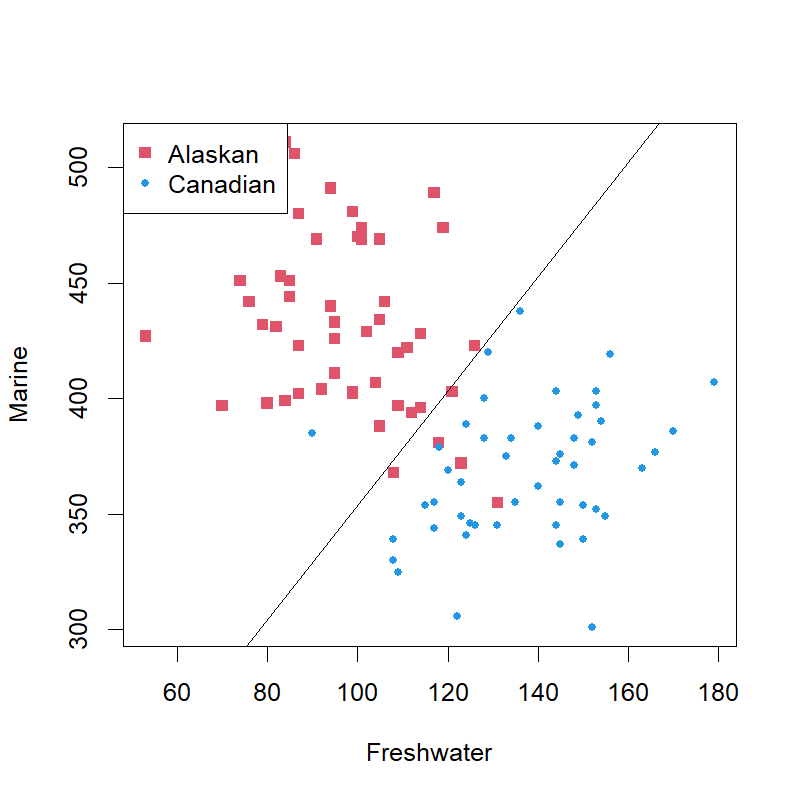
\includegraphics[width=0.7\textwidth]{../Figure/lda_boundary_plot.png}
		\caption{LDA 判别函数决策边界图}
		\label{fig:lda}
	\end{figure}
	
	绘制线性判别函数的决策边界,见图 \ref{fig:lda}.
	\begin{lstlisting}[language=R]
		## 绘制线性判别函数决策边界
		g.mean <- lda.fit$prior %*% lda.fit$means
		const <- as.numeric(g.mean %*% lda.fit$scaling)
		slope <- -lda.fit$scaling[1] / lda.fit$scaling[2]
		intercept <- const / lda.fit$scaling[2]
		plot(salmon[, 2:3],
		pch = rep(c(15, 20), each = 50),
		col = rep(c(2, 4), each = 50)
		)
		abline(intercept, slope)
		legend("topleft",
		legend = c("Alaskan", "Canadian"),
		pch = c(15, 20),
		col = c(2, 4)
		)
	\end{lstlisting}
	由预测结果可知,当线性判别的值为正时,把样本判别为加拿大三文鱼,否则判别为阿拉斯加三文鱼.
	
	从图 \ref{fig:lda} 中可以看出, 线性判别的决策边界是线性函数. LDA方法只能用于协方差矩阵相同的情况,而经过计算可知阿拉斯加和加拿大样本的协方差矩阵差异较大,可以考虑通过QDA方法进行判别,类似地,可以写如下的QDA判别程序:
	\begin{lstlisting}[language=R]
		## QDA函数
		qda.fit <- qda(
		Origin ~ Freshwater + Marine,
		prior = c(1, 1) / 2,
		data = salmon
		)
	\end{lstlisting}
	利用函数\texttt{predict()}进行预测:
	\begin{lstlisting}[language=R]
		## QDA函数
		qda.fit <- qda(
		Origin ~ Freshwater + Marine,
		prior = c(1, 1) / 2,
		data = salmon
		)
	\end{lstlisting}
	得到如下的混淆矩阵:
	
	\begin{table}[ht]
		\caption{三文鱼数据利用QDA的混淆矩阵}
		\centering
		\begin{tabular}{rrr}
			\hline
			& Alaskan & Canadian \\
			\hline
			Alaskan &  45 &   5 \\
			Canadian &   2 &  48 \\
			\hline
		\end{tabular}
	\end{table}
	
	\begin{lstlisting}[language=R]
		## 绘制二次判别函数决策边界
		x <- seq(50, 200, 0.2)
		y <- seq(300, 600, 0.2)
		z <- as.matrix(expand.grid(x, y), 0)
		colnames(z) <- c("Freshwater", "Marine")
		z <- as.data.frame(z)
		m <- length(x)
		n <- length(y)
		z.predict <- as.numeric(predict(object = qda.fit, newdata = z)$class)
		plot(salmon[, 2:3],
		pch = rep(c(15, 20), each = 50),
		col = rep(c(2, 4), each = 50)
		)
		contour(x, y, matrix(z.predict, m, n),
		add = TRUE, drawlabels = FALSE, lty = 1
		)
		legend("topleft",
		legend = c("Alaskan", "Canadian"),
		pch = c(15, 20),
		col = c(2, 4)
		)
	\end{lstlisting}
	\begin{figure}[htbp]
		\centering
		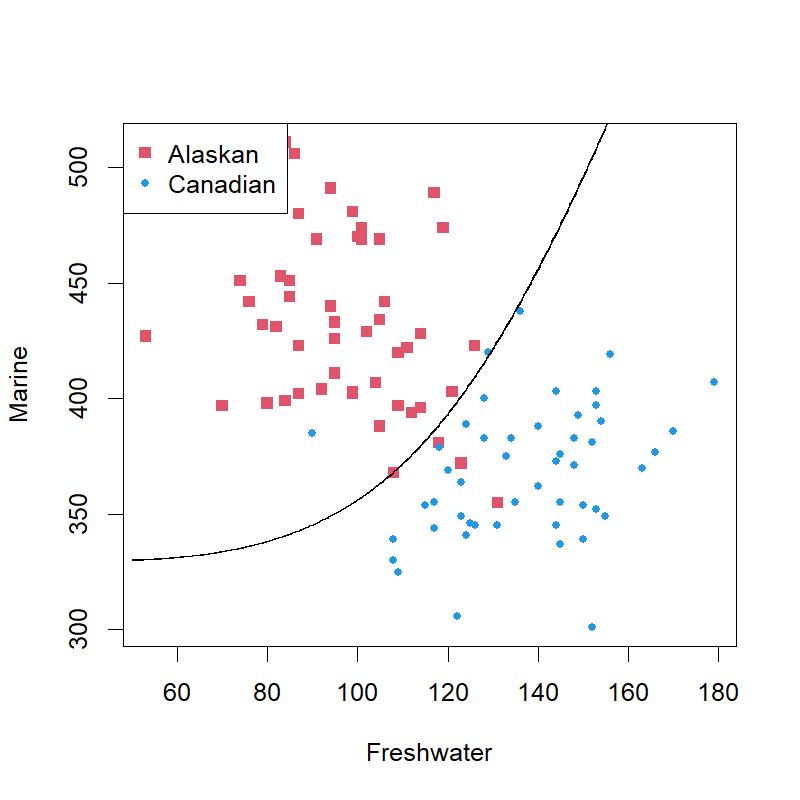
\includegraphics[width=0.7\textwidth]{../Figure/qda_boundary_plot.png}
		\caption{QDA 判别函数决策边界图}
		\label{fig:qda}
	\end{figure}
	从图 \ref{fig:qda} 中可以看出决策边界非线性.
	
	\subsection{Fisher判别法}
	Fisher判别法的思想是把多维数据投影到一维直线上,使得同类数据尽量接近,异类数据尽量分开. 从方差分析角度看,是组内变差要小,组间变差要大.
	
	Fisher判别也要利用距离判别,有线性判别、非线性判别和典型判别等多种常用方法,这里仅讨论线性判别法.
	\subsubsection{两总体Fisher判别}
	设有两个总体 \(G_1\) 和 \(G_2\),求一个向量 \(a \in \mathbb{R}^p\),使得将两个总体投影到该向量方向后,投影结果之间的距离最大. 记 \(G_1, G_2\) 的均值向量分别为 \(\mu_1, \mu_2\),且协方差矩阵均为 \(\Sigma\).
	
	令 \(X^{(1)} \sim G_1\),\(X^{(2)} \sim G_2\),考虑投影变量 \(Y_1 = a^\top X^{(1)}\),\(Y_2 = a^\top X^{(2)}\),则有:
	\[
	\mathbb{E}Y_1 = a^\top \mu_1, \quad \mathbb{E}Y_2 = a^\top \mu_2,
	\]
	\[
	\mathrm{Var}(Y_1) = \mathrm{Var}(Y_2) = a^\top \Sigma a.
	\]
	
	接下来,考虑这两个投影后的均值之间的一维马氏距离,并希望通过选择合适的向量 \(a\),使得该距离最大化. 即需最大化如下目标函数:
	\begin{equation}
		\max_{a \in \mathbb{R}^p} \frac{\left[ a^\top (\mu_1 - \mu_2) \right]^2}{a^\top \Sigma a}.
	\end{equation}
	
	\begin{theorem}
		当 \(a = c \Sigma^{-1} (\mu_1 - \mu_2)\),其中 \(c \neq 0\) 为常数时,上述目标函数取得最大值.
	\end{theorem}
	特别地,当 \(c = 1\) 时,得到的线性判别函数为:
	\begin{equation}
		y = a^\top x = (\mu_1 - \mu_2)^\top \Sigma^{-1} x,
	\end{equation}
	
	该函数称为 \textbf{Fisher 线性判别函数}.
	取
	\[
	\mu_y = \frac{1}{2}(\mathbb{E}Y_1 + \mathbb{E}Y_2) = \frac{1}{2} a^\top (\mu_1 + \mu_2) = \frac{1}{2} (\mu_1 - \mu_2)^\top \Sigma^{-1} (\mu_1 + \mu_2),
	\]
	则
	\[
	\mathbb{E}Y_1 - \mu_y = a^\top \left( \mu_1 - \frac{\mu_1 + \mu_2}{2} \right) = \frac{1}{2} (\mu_1 - \mu_2)^\top \Sigma^{-1} (\mu_1 - \mu_2) > 0,
	\]
	\[
	\mathbb{E}Y_2 - \mu_y = a^\top \left( \mu_2 - \frac{\mu_1 + \mu_2}{2} \right) = -\frac{1}{2} (\mu_1 - \mu_2)^\top \Sigma^{-1} (\mu_1 - \mu_2) < 0.
	\]
	
	于是得到 Fisher 线性判别规则为:
	\[
	\begin{cases}
		\text{判定 } x \in G_1, & \text{如果 } y = (\mu_1 - \mu_2)^\top \Sigma^{-1} x \geq \mu_y, \\
		\text{判定 } x \in G_2, & \text{如果 } y = (\mu_1 - \mu_2)^\top \Sigma^{-1} x < \mu_y.
	\end{cases}
	\]
	
	若定义线性函数
	\begin{equation}
		W(x) = (\mu_1 - \mu_2)^\top \Sigma^{-1} x - \mu_y = (\mu_1 - \mu_2)^\top \Sigma^{-1} \left( x - \frac{\mu_1 + \mu_2}{2} \right),
	\end{equation}
	
	
	则判别规则可进一步写为:
	\[
	\begin{cases}
		\text{判定 } x \in G_1, & \text{如果 } W(x) \geq 0, \\
		\text{判定 } x \in G_2, & \text{如果 } W(x) < 0.
	\end{cases}
	\]
	
	这与在协方差相等条件下马氏距离判别法得到的线性判别函数形式一致.
	\subsubsection{多总体Fisher判别}
	
	在存在多个总体的情形下,需要寻找多个投影方向,以建立多个判别函数。设有 \(k\) 个总体 \(G_1, G_2, \ldots, G_k\),其均值向量分别为 \(\mu_1, \mu_2, \ldots, \mu_k\),共有协方差矩阵为 \(\Sigma\)。设随机向量 \(X^{(j)}\) 来自总体 \(G_j\),考虑向量 \(a \in \mathbb{R}^p\),定义投影变量 \(Y_j = a^\top X^{(j)}\). 记
	\[
	\bar{\mu} = \frac{1}{k} \sum_{j=1}^{k} \mu_j, \quad G = \sum_{j=1}^{k} (\mu_j - \bar{\mu})(\mu_j - \bar{\mu})^\top.
	\]
	
	令 \(\bar{Y} = \frac{1}{k}(Y_1 + Y_2 + \cdots + Y_k)\),则
	\[
	\mu_y = \mathbb{E}(\bar{Y}) = a^\top \bar{\mu}.
	\]
	
	考虑 \(\mathbb{E}Y_j\) 与 \(\mu_y\) 的一维马氏距离平方,即
	\[
	\frac{(\mathbb{E}Y_j - \mu_y)^2}{\mathrm{Var}(Y_j)} = \frac{[a^\top(\mu_j - \bar{\mu})]^2}{a^\top \Sigma a}, \quad j = 1, 2, \ldots, k.
	\]
	
	令这 \(k\) 个平方距离的和最大,即
	
	\begin{equation}
		\max_{a \in \mathbb{R}^p} \frac{\sum_{j=1}^{k} a^\top(\mu_j - \bar{\mu})(\mu_j - \bar{\mu})^\top a}{a^\top \Sigma a} = \frac{a^\top G a}{a^\top \Sigma a}. \label{maximumdistance}
	\end{equation}
	
	
	因此,若在向量 \(a\) 方向上投影,则类别间距离最远.
	
	\begin{theorem}
		设 \(\Sigma^{-1} G\) 的非零特征值为 \(\lambda_1 \geq \lambda_2 \geq \cdots \geq \lambda_s\)(其中 \(s \leq \min(k-1, p)\)),相应的特征向量为 \(e_1, e_2, \ldots, e_s\),且满足 \(e_i^\top \Sigma e_i = 1\)。当 \(a = e_1\) 时,\eqref{maximumdistance} 达到最大值,称 \(e_1^\top x\) 为第一判别函数. 当 \(a = e_2\) 且满足 \(\mathrm{Cov}(e_1^\top X, a^\top X) = 0\) 时,\eqref{maximumdistance} 达到次大值,称 \(e_2^\top x\) 为第二判别函数.依此类推,当 \(a = e_j\) 且满足 \(\mathrm{Cov}(e_i^\top X, a^\top X) = 0\) 对 \(i = 1, 2, \ldots, j-1\) 成立时,上式达到第 \(j\) 大值,称 \(e_j^\top x\) 为第 \(j\) 判别函数.
	\end{theorem}
	
	\subsubsection{代码实践}
	\begin{example}
		R中iris数据包含三个类(Species),每类50个样品. 每个观测有花萼长、宽与花瓣长、宽计四个测量值,以此作为训练集.		
	\end{example}
	Fisher判别法将数据投影到分辨力最高的方向上,进行判别. 在R中用\texttt{MASS::lda()}函数,也称线性判别. 用\texttt{predict()}进行判别. 用\texttt{table()}列表训练准确程度. 
	这里需要使用\texttt{prior=}指定一个各类相等的先验概率,如这里需要\text{prior=rep(1/3, 3)}.
	
	用150个样本点估计判别函数:
	\begin{lstlisting}[language=R]
		library(MASS)
		lda1 <- lda(
		Species ~ Sepal.Length + Sepal.Width + Petal.Length + Petal.Width,
		prior = rep(1 / 3, 3), data = iris
		)
		print(lda1)
	\end{lstlisting}
	
	用训练的模型对参与估计的150个样本点每个进行判别. 结果见附录.
	\begin{lstlisting}[language=R]
		res1 <- predict(lda1)
		print(res1)
	\end{lstlisting}
	
	下面对比用判别函数判别的结果与真实的类属的关系:
	\begin{lstlisting}[language=R]
		newG <- res1$class
		tab <- table(iris$Species, newG)
	\end{lstlisting}
	\begin{table}

		\caption{鸢尾花数据LDA混淆矩阵}
		\centering
		\begin{tabular}[t]{l|r|r|r}
			\hline
			& setosa & versicolor & virginica\\
			\hline
			setosa & 50 & 0 & 0\\
			\hline
			versicolor & 0 & 48 & 2\\
			\hline
			virginica & 0 & 1 & 49\\
			\hline
		\end{tabular}
		\label{table:IrisLDA}
	\end{table}
	输出混淆矩阵表 \ref{table:IrisLDA} . 表中显示仅分错了三例,找出三例.
	\begin{lstlisting}[language=R]
		kable(cbind(iris, Predicted = newG)[iris$Species != newG, ],
		format = "latex", caption = "分类错误样本"
		)
	\end{lstlisting}
	错分的数据见表 \ref{table:misclassify}.
	\begin{table}
		
		\caption{分类错误样本}
		\centering
		\begin{tabular}[t]{l|r|r|r|r|l|l}
			\hline
			& Sepal.Length & Sepal.Width & Petal.Length & Petal.Width & Species & Predicted\\
			\hline
			71 & 5.9 & 3.2 & 4.8 & 1.8 & versicolor & virginica\\
			\hline
			84 & 6.0 & 2.7 & 5.1 & 1.6 & versicolor & virginica\\
			\hline
			134 & 6.3 & 2.8 & 5.1 & 1.5 & virginica & versicolor\\
			\hline
		\end{tabular}
		\label{table:misclassify}
	\end{table}
	\section{支持向量机}
	\subsection{原理简介}
	
	支持向量机(Support Vector Machines, SVM)是一种用于解决二分类问题的监督学习方法,其基本思想是在特征空间中寻找一个能够最大间隔分隔两类样本的超平面. 若数据在特征空间中线性可分,SVM 寻找使分类间隔最大的分离超平面;若不可分,则引入软间隔策略和核函数方法以增强模型的适应能力.
	
	在$p$维空间中,一个超平面是一个维度为$p-1$的仿射子空间,其一般形式为:
	\[
	\beta_0 + \beta_1X_1 + \beta_2X_2 + \cdots + \beta_pX_p = 0
	\]
	其中$\beta=(\beta_1,\beta_2,\cdots,\beta_p)$是法向量,垂直于超平面,$\beta_0$控制平移.
	
	 对于一个点$X$,其在超平面一侧满足$f(X) = \beta_0 + \sum_{j=1}^p \beta_jX_j > 0$,另一侧为$f(X) < 0$. 若我们令$Y_i \in \{-1, +1\}$,则分离超平面需要满足:
	\[
	Y_i \cdot f(X_i) > 0
	\]
	
	最大间隔分类器的问题可以表述为如下的约束优化问题:
	\[
	\begin{aligned}
		& \max_{\beta_0, \beta_1, \ldots, \beta_p} M \\
		 \text{subject to} \quad \sum_{j=1}^{p} \beta_j^2 = 1, \quad &y_i(\beta_0 + \sum_{j=1}^{p} \beta_j x_{ij}) \geq M, \quad \forall i = 1,\ldots,N
	\end{aligned}
	\]
	该问题可以转化为一个凸二次规划问题求解,R语言中e1071包的 \texttt{svm()} 函数可以高效解决。
	
	当数据线性不可分或存在噪声时,引入松弛变量$\varepsilon_i$以允许部分误分类,构成支持向量分类器,其优化形式为:
	\[
	\begin{aligned}
		& \max_{\beta_0, \beta_1, \ldots, \beta_p, \varepsilon_1, \ldots, \varepsilon_n} M \\
		& \text{subject to} \quad \sum_{j=1}^{p} \beta_j^2 = 1, \quad y_i(\beta_0 + \sum_{j=1}^{p} \beta_j x_{ij}) \geq M(1 - \varepsilon_i), \\
		& \varepsilon_i \geq 0, \quad \sum_{i=1}^{n} \varepsilon_i \leq C
	\end{aligned}
	\]
	其中$C$为正则化参数,控制间隔最大化与分类错误之间的权衡. 
	
	调节参数$C$控制将严格要求所有点在正确一侧且不能进入分隔区域的要求放松到多大程度. 当$C = 0$时对应于最大分隔边界判别法,不能有任何点在错误一侧,也不能进入分隔边界区域. 增大$C$的值, 解出的边界宽度也会增大. 过大的$C$使得错判点较多,结果方差较小,偏差较大;过小的$C$使得结果不稳健,预测方差较大,偏差较小. 所以,这里的调节参数与其它有监督学习方法中的调节参数类似,应该在偏差与方差之间折衷,可以用交叉验证方法求最优调节参数值. $C$越小,模型复杂度越高.
	
	若线性分割无法完成分类任务,则可以通过特征扩展将原始特征映射至更高维空间,解决非线性问题的常用方法是增加非线性项如二次项、三次项. 例如,将自变量由 \(x_1, \ldots, x_p\) 增加到
	\[
	x_1, \ldots, x_p, x_1^2, \ldots, x_p^2,
	\]
	则支持向量判别法的优化问题变成了
	\[
	\max_{\beta_0, \beta_{11}, \ldots, \beta_{p1}, \beta_{12}, \ldots, \beta_{p2}, \epsilon_1, \ldots, \epsilon_n} \quad \text{M} \quad \text{s.t.}
	\]
	\[
	y_i \left( \beta_0 + \sum_{j=1}^{p} \beta_{j1} x_{ij} + \sum_{j=1}^{p} \beta_{j2} x_{ij}^2 \right) \geq \text{M} \times (1 - \epsilon_i), \quad i = 1, 2, \ldots, n,
	\]
	\[
	\sum_{k=1}^{2} \sum_{j=1}^{p} \beta_{jk}^2 = 1, \quad \varepsilon_i \geq 0, \quad \sum_{i=1}^{n} \varepsilon_i \leq C.
	\]
	
	这样得到的边界在 \((x_1, \ldots, x_p, x_1^2, \ldots, x_p^2)\) 所在的 \(\mathbb{R}^{2p}\) 空间内是线性的超平面,但在原来的 \((x_1, \ldots, x_p)\) 所在的 \(\mathbb{R}^p\) 空间中则是由 \(q(x) = 0\) 决定的曲面,其中 \(q(x)\) 是二次多项式函数。
	
	还可以增加高次项甚至交叉项,或者考虑其他更复杂的非线性变换. 增加非线性项的方法有无数种,且一一测试并不现实,支持向量机方法则给出了一种增加非线性项的一般方法,使得对应的边界可以快速求解.
	
	核方法(Kernel Trick)提供了一种无需显式扩展特征空间的方法,利用了 Hilbert 空间的方法将线性问题扩展为非线性问题. 线性的支持向量判别法可以通过 \(\mathbb{R}^p\) 的内积转化为如下的等价方法:
	
	判别函数可以表示为:
	\[
	f(x) = \beta_0 + \sum_{i=1}^{n} \alpha_i \langle x, x_i \rangle,
	\]
	其中 \(\beta_0, \alpha_1, \ldots, \alpha_n\) 是待估参数。为了估计参数,不需要用到各 \(x_i\) 的具体值,而只需其两两间的内积值. 又判别函数中只有支持向量对应的 \(\alpha_i\) 非零,记 \(S\) 为支持向量点集,则线性判别函数为:
	\[
	f(x) = \beta_0 + \sum_{i \in S} \alpha_i \langle x, x_i \rangle.
	\]
	
	支持向量方法将 \(\mathbb{R}^p\) 中的内积推广为如下的核函数值,例如
	\[
	K(x, x') = \sum_{j=1}^{p} x_j x_j',
	\]
	其中 \(K(x, x')\), \(x, x' \in \mathbb{R}^p\),是度量两个观测点 \(x, x'\) 的相似程度的函数. 该定义核函数的形式即为线性核,从而回到了线性的支持向量判别方法.
	
	利用核代替内积后,判别法的判别函数变成:
	\[
	f(x) = \beta_0 + \sum_{i \in S} \alpha_i K(x, x_i).
	\]
	
	核函数有多种形式. 例如,取多项式核函数:
	\[
	K(x, x') = \left( 1 + \sum_{j=1}^{p} x_j x_j' \right)^d,
	\]
	其中 \(d > 1\) 为正整数. 称为\textbf{多项式核},本质上是对线性的支持向量方法添加了高次项及其交叉项.
	
	当 \(d = 2\) 时,核函数形式为:
	\[
	K(x, x') = \left(1 + \sum_{j=1}^{p} x_j x_j' \right)^2.
	\]
	可以看出,增加了二次项及交叉项. 将 \(x\) 空间映射为
	\[
	\phi(x) = (x_1, x_2, \ldots, x_p, x_1^2, x_2^2, \ldots, x_p^2, x_1 x_2, \ldots),
	\]
	即将原始空间 \(\mathbb{R}^p\) 的点映射至高维空间中的分隔超平面,在原空间中该超平面对应的是非线性曲面.
	
	如此一来,判别函数实质上在高维 \(\mathbb{R}^{2p}\) 中是线性的,但其在原始空间 \(\mathbb{R}^p\) 中表现为非线性函数:
	\[
	f(x) = \beta_0 + \sum_{i \in S} \alpha_i \langle \phi(x), \phi(x_i) \rangle = \beta_0 + \sum_{i \in S} \alpha_i K(x, x_i).
	\]
	
	理论研究表明,给定核函数 \(K(\cdot, \cdot)\) 后,必存在某个 Hilbert 空间 \(H\) 和映射 \(\phi(x) \in H\),使得
	\[
	K(x, x') = \langle \phi(x), \phi(x') \rangle_H.
	\]
	
	于是,给定一个核函数,就可以将原本的 \(\mathbb{R}^p\) 空间中的非线性判别问题,转化为 \(H\) 空间中的线性判别问题. 这样得出的判别函数在 \(H\) 空间中是线性的,但在原始的 \(\mathbb{R}^p\) 空间中却是非线性的.
	
	训练这样的支持向量机模型时,只需计算两两之间的核函数值 \(K(x, x')\),而无需显式地计算映射后的 \(\phi(x)\). 这也解释了为何不直接增加非线性项:一方面核函数的计算更高效,另一方面高维空间的映射可能导致维数升高,显式表示 \(\phi(x)\) 不切实际.
	
	
	另一种常用的核是径向基核(radial kernel),其定义为:
	\[
	K(x, x') = \exp \left( -\gamma \sum_{j=1}^{p} (x_j - x'_j)^2 \right),
	\]
	其中 \(\gamma\) 是正数. 
	
	对应的判别函数可写为:
	\[
	f(x) = \beta_0 + \sum_{i \in S} \alpha_i \exp \left( -\gamma \sum_{j=1}^{p} (x_j - x_{ij})^2 \right).
	\]
	
	对一个特定的观测样本 \(x^*\),如果它与训练样本 \(x_i\) 相距较远,则 \(K(x^*, x_i)\) 很小,其 \(\alpha_i\) 对 \(x^*\) 的判别影响极小;反之,则影响较大. 这样的核函数使得径向基核具有很强的局部性,只有靠近的样本才对判别起作用.
	
	\subsection{代码实践}
	\begin{example}
		数据集Heart中有303个病人的数据,其中变量AHD是二值变量,取Yes表示用血管造影检查确诊心脏病的,No表示没有心脏病的. 有13个自变量,包括Age, Sex, Chol(胆固醇化验指标)等.
	\end{example}
	\subsubsection{LDA vs SVC}
	训练集上同时使用线性判别法(LDA)和支持向量判别法(SVC).
	\begin{lstlisting}[language=R]
		library(e1071)
		library(ROCR)
		library(MASS)
		
		## 读取Heart数据
		Heart <- read.csv(
		"Heart.csv",
		header = TRUE, row.names = 1,
		stringsAsFactors = TRUE
		)
		d <- na.omit(Heart)
		set.seed(1)
		train_id <- sample(nrow(d), size = round(0.7 * nrow(d)))
		train <- rep(FALSE, nrow(d))
		train[train_id] <- TRUE
		test <- (!train)
		d[["AHD"]] <- factor(d[["AHD"]], levels = c("No", "Yes"))
	\end{lstlisting}
	
	定义错判率函数:
	\begin{lstlisting}[language=R]
		## 定义错判率函数
		classifier.error <- function(truth, pred) {
			tab1 <- table(truth, pred)
			err <- 1 - sum(diag(tab1)) / sum(c(tab1))
			err
		}
	\end{lstlisting}
	
	进行线性判别:
	\begin{lstlisting}[language=R]
		res.ld <- lda(AHD ~ ., data = d[train, ], prior = rep(1 / 2, 2))
	\end{lstlisting}
	
	进行支持向量判别法,即SVM取多项式核,阶数$d=1$的情形. 此时需要一个调节参数cost,cost越大,分隔边界越窄,越容易导致过拟合.
	\begin{lstlisting}[language=R]
		res.svc <- svm(
		AHD ~ .,
		data = d[train, ],
		kernel = "linear", cost = 1, scale = TRUE
		)
		fit.svc <- predict(res.svc)
		tab1 <- table(truth = d[train, "AHD"], fitted = fit.svc)
	\end{lstlisting}
	
	\texttt{e1071}函数提供了\texttt{tune()}函数,可以在训练集上用十折交叉验证选择较好的调节参数.
	\begin{lstlisting}[language=R]
		set.seed(101)
		res.tune <- tune(
		svm, AHD ~ .,
		data = d[train, ], kernel = "linear", scale = TRUE,
		ranges = list(cost = c(0.001, 0.01, 0.1, 1, 5, 10, 100, 1000))
		)
	\end{lstlisting}
	
	在测试集上测试两种方法.
	\begin{lstlisting}[language=R]
		pred.ld <- predict(res.ld, d[test, ])$class
		tab1 <- table(truth = d[test, "AHD"], predict = pred.ld)
		pred.svc <- predict(res.tune$best.model, newdata = d[test, ])
		tab1 <- table(truth = d[test, "AHD"], predict = pred.svc)
	\end{lstlisting}
	
	绘制在Heart训练集上LDA和SVC的ROC曲线.
	\begin{lstlisting}[language=R]
		png(filename = "roc_curve_training.png", width = 800, height = 600)
		pred.ld <- predict(res.ld,
		newdata = d[train, ],
		decision.values = TRUE
		)
		decf.ld <- pred.ld$posterior[, "Yes"]
		predobj <- prediction(decf.ld, d[train, "AHD"],
		label.ordering = c("No", "Yes")
		)
		perf <- performance(predobj, "tpr", "fpr")
		plot(perf, main = "ROC Curve (Training Data)", col = "cyan")
		
		pred.svc <- predict(
		res.tune$best.model,
		newdata = d[train, ],
		decision.values = TRUE
		)
		decf.svc <- attributes(pred.svc)$decision.values
		predobj <- prediction(
		decf.svc, d[train, "AHD"],
		label.ordering = c("No", "Yes")
		)
		perf <- performance(predobj, "tpr", "fpr")
		plot(perf, add = TRUE, col = "blue")
		legend("bottomright",
		lty = 1, col = c("cyan", "blue"),
		legend = c("LDA", "SVC")
		)
		dev.off()
	\end{lstlisting}
	从图 \ref{fig:roc_curve} 中可以看出,两种方法效果相近.
	\begin{figure}[htbp]
		\centering
		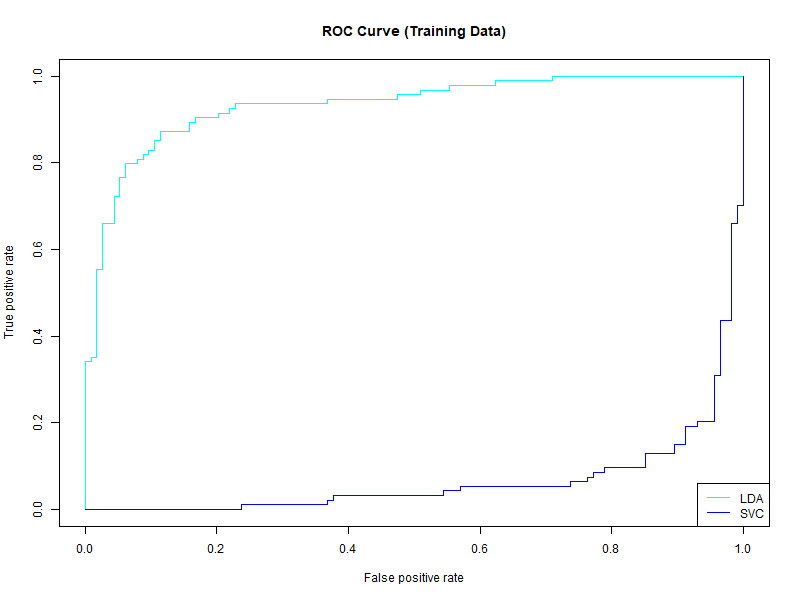
\includegraphics[width=0.8\textwidth]{../Figure/roc_curve_training.png}
		\caption{ROC Curve for Training Data (LDA vs. SVC)}
		\label{fig:roc_curve}
	\end{figure}
	\subsubsection{多项式SVM}
	
	用多项式核的SVM建模:
	\begin{lstlisting}[language=R]
		## 多项式核SVM
		res.svm1 <- svm(AHD ~ .,
		data = d[train, ], kernel = "polynomial",
		order = 2, cost = 0.1, scale = TRUE
		)
		fit.svm1 <- predict(res.svm1)
		tab1 <- table(truth = d[train, "AHD"], fitted = fit.svm1)
	\end{lstlisting}
	
	寻找最优参数,并且用于测试集:
	\begin{lstlisting}[language=R]
		set.seed(101)
		res.tune2 <- tune(
		svm, AHD ~ .,
		data = d[train, ], kernel = "polynomial",
		order = 2, scale = TRUE,
		ranges = list(cost = c(0.001, 0.01, 0.1, 1, 5, 10, 100, 1000))
		)
		fit.svm2 <- predict(res.tune2$best.model)
		tab1 <- table(truth = d[train, "AHD"], fitted = fit.svm2)
		pred.svm2 <- predict(res.tune2$best.model, d[test, ])
		tab1 <- table(truth = d[test, "AHD"], predict = pred.svm2)
	\end{lstlisting}
	
	\subsubsection{径向核SVM}
	
	用径向核的SVM建模:
	\begin{lstlisting}[language=R]
		## 径向核SVM
		res.svm3 <- svm(
		AHD ~ .,
		data = d[train, ], kernel = "radial",
		gamma = 0.1, cost = 0.1, scale = TRUE
		)
		fit.svm3 <- predict(res.svm3)
		tab1 <- table(truth = d[train, "AHD"], fitted = fit.svm3)
	\end{lstlisting}
	
	寻找最优参数,并且用于测试集:
	\begin{lstlisting}[language=R]
		set.seed(101)
		res.tune4 <- tune(
		svm, AHD ~ .,
		data = d[train, ], kernel = "radial",
		scale = TRUE,
		ranges = list(
		cost = c(0.001, 0.01, 0.1, 1, 5, 10, 100, 1000),
		gamma = c(0.1, 0.01, 0.001)
		)
		)
		fit.svm4 <- predict(res.tune4$best.model)
		tab1 <- table(truth = d[train, "AHD"], fitted = fit.svm4)
		pred.svm4 <- predict(res.tune4$best.model, d[test, ])
		tab1 <- table(truth = d[test, "AHD"], predict = pred.svm2)
	\end{lstlisting}
	\newpage
	
	\begin{thebibliography}{99}
		\bibitem{a}李高荣,吴密霞 编著. \emph{多元统计分析}[M]. 北京: 科学出版社, 2021.
		\bibitem{b}高惠璇. \emph{应用多元统计分析}[M].北京大学出版社,2005.
		\bibitem{c}James, Gareth, Daniela Witten, Trevor Hastie, and Robert Tibshirani. 2013. An Introduction to Statistical Learning with Applications in r. Springer.
	\end{thebibliography}
	
	\newpage
	
	\begin{appendices}
		\renewcommand{\thesection}{\Alph{section}}
		\section{部分程序输出}
	\begin{lstlisting}[language=R, caption={训练好的模型对鸢尾花数据集的预测结果}, label=predictIris]
		$class
		[1] setosa     setosa     setosa     setosa     setosa     setosa
		[7] setosa     setosa     setosa     setosa     setosa     setosa
		[13] setosa     setosa     setosa     setosa     setosa     setosa
		[19] setosa     setosa     setosa     setosa     setosa     setosa
		[25] setosa     setosa     setosa     setosa     setosa     setosa
		[31] setosa     setosa     setosa     setosa     setosa     setosa
		[37] setosa     setosa     setosa     setosa     setosa     setosa
		[43] setosa     setosa     setosa     setosa     setosa     setosa
		[49] setosa     setosa     versicolor versicolor versicolor versicolor
		[55] versicolor versicolor versicolor versicolor versicolor versicolor
		[61] versicolor versicolor versicolor versicolor versicolor versicolor
		[67] versicolor versicolor versicolor versicolor virginica  versicolor
		[73] versicolor versicolor versicolor versicolor versicolor versicolor
		[79] versicolor versicolor versicolor versicolor versicolor virginica
		[85] versicolor versicolor versicolor versicolor versicolor versicolor
		[91] versicolor versicolor versicolor versicolor versicolor versicolor
		[97] versicolor versicolor versicolor versicolor virginica  virginica
		[103] virginica  virginica  virginica  virginica  virginica  virginica
		[109] virginica  virginica  virginica  virginica  virginica  virginica
		[115] virginica  virginica  virginica  virginica  virginica  virginica
		[121] virginica  virginica  virginica  virginica  virginica  virginica
		[127] virginica  virginica  virginica  virginica  virginica  virginica
		[133] virginica  versicolor virginica  virginica  virginica  virginica
		[139] virginica  virginica  virginica  virginica  virginica  virginica
		[145] virginica  virginica  virginica  virginica  virginica  virginica
		Levels: setosa versicolor virginica
		
		$posterior
		setosa   versicolor    virginica
		1   1.000000e+00 3.896358e-22 2.611168e-42
		2   1.000000e+00 7.217970e-18 5.042143e-37
		3   1.000000e+00 1.463849e-19 4.675932e-39
		4   1.000000e+00 1.268536e-16 3.566610e-35
		5   1.000000e+00 1.637387e-22 1.082605e-42
		6   1.000000e+00 3.883282e-21 4.566540e-40
		7   1.000000e+00 1.113469e-18 2.302608e-37
		8   1.000000e+00 3.877586e-20 1.074496e-39
		9   1.000000e+00 1.902813e-15 9.482936e-34
		10  1.000000e+00 1.111803e-18 2.724060e-38
		11  1.000000e+00 1.185277e-23 3.237084e-44
		12  1.000000e+00 1.621649e-18 1.833201e-37
		13  1.000000e+00 1.459225e-18 3.262506e-38
		14  1.000000e+00 1.117219e-19 1.316642e-39
		15  1.000000e+00 5.487399e-30 1.531265e-52
		16  1.000000e+00 1.261505e-27 2.268705e-48
		17  1.000000e+00 6.754338e-25 3.868271e-45
		18  1.000000e+00 4.223741e-21 1.224313e-40
		19  1.000000e+00 1.774911e-22 2.552153e-42
		20  1.000000e+00 2.593237e-22 5.792079e-42
		21  1.000000e+00 1.274639e-19 4.357774e-39
		22  1.000000e+00 1.465999e-20 1.987241e-39
		23  1.000000e+00 6.569280e-25 7.769177e-46
		24  1.000000e+00 8.912348e-15 9.178624e-32
		25  1.000000e+00 1.070702e-15 1.167516e-33
		26  1.000000e+00 2.497339e-16 5.710269e-35
		27  1.000000e+00 3.967732e-17 4.378624e-35
		28  1.000000e+00 1.548165e-21 1.595360e-41
		29  1.000000e+00 9.271847e-22 6.297955e-42
		30  1.000000e+00 9.665144e-17 2.977974e-35
		31  1.000000e+00 2.299936e-16 7.182666e-35
		32  1.000000e+00 1.975404e-19 2.788334e-38
		33  1.000000e+00 7.100041e-27 2.216408e-48
		34  1.000000e+00 1.610295e-28 2.743783e-50
		35  1.000000e+00 1.205219e-17 1.277245e-36
		36  1.000000e+00 1.597186e-21 9.033772e-42
		37  1.000000e+00 1.939869e-24 1.662808e-45
		38  1.000000e+00 3.310234e-23 7.004971e-44
		39  1.000000e+00 4.190242e-17 6.991441e-36
		40  1.000000e+00 1.769359e-20 3.541694e-40
		41  1.000000e+00 1.063014e-21 2.003866e-41
		42  1.000000e+00 2.174217e-11 1.213781e-28
		43  1.000000e+00 1.540753e-18 1.305719e-37
		44  1.000000e+00 8.940589e-16 1.315511e-32
		45  1.000000e+00 1.616206e-17 3.205992e-35
		46  1.000000e+00 1.714743e-16 7.172435e-35
		47  1.000000e+00 2.083089e-22 2.289783e-42
		48  1.000000e+00 2.793482e-18 2.629539e-37
		49  1.000000e+00 2.597560e-23 9.820820e-44
		50  1.000000e+00 2.322258e-20 4.241757e-40
		51  1.969732e-18 9.998894e-01 1.105878e-04
		52  1.242878e-19 9.992575e-01 7.425297e-04
		53  2.088263e-22 9.958069e-01 4.193053e-03
		54  2.198898e-22 9.996423e-01 3.576502e-04
		55  4.213678e-23 9.955903e-01 4.409655e-03
		56  8.127287e-23 9.985020e-01 1.497982e-03
		57  3.549900e-22 9.858346e-01 1.416542e-02
		58  5.007065e-14 9.999999e-01 1.119811e-07
		59  5.683334e-20 9.998781e-01 1.218649e-04
		60  1.241039e-20 9.995027e-01 4.973085e-04
		61  1.956628e-18 9.999986e-01 1.420841e-06
		62  5.968900e-20 9.992294e-01 7.705716e-04
		63  2.716128e-18 9.999988e-01 1.220169e-06
		64  1.184445e-23 9.943267e-01 5.673286e-03
		65  5.574931e-14 9.999984e-01 1.649215e-06
		66  2.369511e-17 9.999573e-01 4.268212e-05
		67  8.429328e-24 9.806471e-01 1.935289e-02
		68  2.505072e-16 9.999991e-01 9.151716e-07
		69  1.670352e-27 9.595735e-01 4.042653e-02
		70  1.341503e-17 9.999967e-01 3.296105e-06
		71  7.408118e-28 2.532282e-01 7.467718e-01
		72  9.399292e-17 9.999907e-01 9.345291e-06
		73  7.674672e-29 8.155328e-01 1.844672e-01
		74  2.683018e-22 9.995723e-01 4.277469e-04
		75  7.813875e-18 9.999758e-01 2.421458e-05
		76  2.073207e-18 9.999171e-01 8.290530e-05
		77  6.357538e-23 9.982541e-01 1.745936e-03
		78  5.639473e-27 6.892131e-01 3.107869e-01
		79  3.773528e-23 9.925169e-01 7.483138e-03
		80  9.555338e-12 1.000000e+00 1.910624e-08
		81  1.022109e-17 9.999970e-01 3.007748e-06
		82  9.648075e-16 9.999997e-01 3.266704e-07
		83  1.616405e-16 9.999962e-01 3.778441e-06
		84  4.241952e-32 1.433919e-01 8.566081e-01
		85  1.724514e-24 9.635576e-01 3.644242e-02
		86  1.344746e-20 9.940401e-01 5.959931e-03
		87  3.304868e-21 9.982223e-01 1.777672e-03
		88  2.034571e-23 9.994557e-01 5.443096e-04
		89  5.806986e-18 9.999486e-01 5.137101e-05
		90  5.981190e-21 9.998183e-01 1.816870e-04
		91  5.878614e-23 9.993856e-01 6.144200e-04
		92  5.399006e-22 9.980934e-01 1.906591e-03
		93  3.559507e-18 9.999887e-01 1.128570e-05
		94  2.104146e-14 9.999999e-01 1.135016e-07
		95  4.700877e-21 9.996980e-01 3.020226e-04
		96  1.584328e-17 9.999817e-01 1.826327e-05
		97  2.802293e-19 9.998892e-01 1.108315e-04
		98  1.626918e-18 9.999536e-01 4.640488e-05
		99  7.638378e-11 1.000000e+00 1.867332e-08
		100 4.679301e-19 9.999269e-01 7.305863e-05
		101 7.503075e-52 7.127303e-09 1.000000e+00
		102 5.213802e-38 1.078251e-03 9.989217e-01
		103 1.231264e-42 2.592826e-05 9.999741e-01
		104 1.537499e-38 1.068139e-03 9.989319e-01
		105 6.242501e-46 1.812963e-06 9.999982e-01
		106 4.209281e-49 6.656263e-07 9.999993e-01
		107 3.797837e-33 4.862025e-02 9.513797e-01
		108 1.352176e-42 1.395463e-04 9.998605e-01
		109 1.323390e-42 2.235313e-04 9.997765e-01
		110 3.453358e-46 1.727277e-07 9.999998e-01
		111 5.452660e-32 1.305353e-02 9.869465e-01
		112 1.182560e-37 1.673875e-03 9.983261e-01
		113 5.204321e-39 2.006352e-04 9.997994e-01
		114 1.269953e-40 1.948672e-04 9.998051e-01
		115 1.685361e-45 1.000455e-06 9.999990e-01
		116 5.141640e-40 2.605493e-05 9.999739e-01
		117 1.909820e-35 6.083553e-03 9.939164e-01
		118 1.207799e-44 1.503799e-06 9.999985e-01
		119 3.181265e-59 1.317279e-09 1.000000e+00
		120 1.598511e-33 2.207990e-01 7.792010e-01
		121 1.119461e-42 6.451865e-06 9.999935e-01
		122 3.038170e-37 8.272676e-04 9.991727e-01
		123 6.032879e-50 9.509838e-07 9.999990e-01
		124 1.951261e-31 9.711942e-02 9.028806e-01
		125 1.956408e-39 8.836845e-05 9.999116e-01
		126 1.109337e-36 2.679310e-03 9.973207e-01
		127 7.841997e-30 1.883675e-01 8.116325e-01
		128 7.964690e-30 1.342431e-01 8.657569e-01
		129 6.190641e-44 1.303681e-05 9.999870e-01
		130 1.406448e-32 1.036823e-01 8.963177e-01
		131 4.108129e-42 1.442338e-04 9.998558e-01
		132 1.555697e-36 5.198047e-04 9.994802e-01
		133 1.320330e-45 3.014091e-06 9.999970e-01
		134 1.283891e-28 7.293881e-01 2.706119e-01
		135 1.926560e-35 6.602253e-02 9.339775e-01
		136 1.271083e-45 2.152818e-06 9.999978e-01
		137 3.038963e-44 8.881859e-07 9.999991e-01
		138 4.605973e-35 6.165648e-03 9.938344e-01
		139 4.538634e-29 1.925262e-01 8.074738e-01
		140 2.140232e-36 8.290895e-04 9.991709e-01
		141 6.570902e-45 1.180810e-06 9.999988e-01
		142 6.202588e-36 4.276398e-04 9.995724e-01
		143 5.213802e-38 1.078251e-03 9.989217e-01
		144 1.073945e-45 1.028519e-06 9.999990e-01
		145 4.048249e-46 2.524984e-07 9.999997e-01
		146 4.970070e-39 7.473361e-05 9.999253e-01
		147 4.616611e-36 5.898784e-03 9.941012e-01
		148 5.548962e-35 3.145874e-03 9.968541e-01
		149 1.613687e-40 1.257468e-05 9.999874e-01
		150 2.858012e-33 1.754229e-02 9.824577e-01
		
		$x
		LD1          LD2
		1    8.0617998 -0.300420621
		2    7.1286877  0.786660426
		3    7.4898280  0.265384488
		4    6.8132006  0.670631068
		5    8.1323093 -0.514462530
		6    7.7019467 -1.461720967
		7    7.2126176 -0.355836209
		8    7.6052935  0.011633838
		9    6.5605516  1.015163624
		10   7.3430599  0.947319209
		11   8.3973865 -0.647363392
		12   7.2192969  0.109646389
		13   7.3267960  1.072989426
		14   7.5724707  0.805464137
		15   9.8498430 -1.585936985
		16   9.1582389 -2.737596471
		17   8.5824314 -1.834489452
		18   7.7807538 -0.584339407
		19   8.0783588 -0.968580703
		20   8.0209745 -1.140503656
		21   7.4968023  0.188377220
		22   7.5864812 -1.207970318
		23   8.6810429 -0.877590154
		24   6.2514036 -0.439696367
		25   6.5589334  0.389222752
		26   6.7713832  0.970634453
		27   6.8230803 -0.463011612
		28   7.9246164 -0.209638715
		29   7.9912902 -0.086378713
		30   6.8294645  0.544960851
		31   6.7589549  0.759002759
		32   7.3749525 -0.565844592
		33   9.1263463 -1.224432671
		34   9.4676820 -1.825226345
		35   7.0620139  0.663400423
		36   7.9587624  0.164961722
		37   8.6136720 -0.403253602
		38   8.3304176 -0.228133530
		39   6.9341201  0.705519379
		40   7.6882313  0.009223623
		41   7.9179372 -0.675121313
		42   5.6618807  1.934355243
		43   7.2410147  0.272615132
		44   6.4144356 -1.247301306
		45   6.8594438 -1.051653957
		46   6.7647039  0.505151855
		47   8.0818994 -0.763392750
		48   7.1867690  0.360986823
		49   8.3144488 -0.644953177
		50   7.6719674  0.134893840
		51  -1.4592755 -0.028543764
		52  -1.7977057 -0.484385502
		53  -2.4169489  0.092784031
		54  -2.2624735  1.587252508
		55  -2.5486784  0.472204898
		56  -2.4299673  0.966132066
		57  -2.4484846 -0.795961954
		58  -0.2226665  1.584673183
		59  -1.7502012  0.821180130
		60  -1.9584224  0.351563753
		61  -1.1937603  2.634455704
		62  -1.8589257 -0.319006544
		63  -1.1580939  2.643409913
		64  -2.6660572  0.642504540
		65  -0.3783672 -0.086638931
		66  -1.2011726 -0.084437359
		67  -2.7681025 -0.032199536
		68  -0.7768540  1.659161847
		69  -3.4980543  1.684956162
		70  -1.0904279  1.626583496
		71  -3.7158961 -1.044514421
		72  -0.9976104  0.490530602
		73  -3.8352593  1.405958061
		74  -2.2574125  1.426794234
		75  -1.2557133  0.546424197
		76  -1.4375576  0.134424979
		77  -2.4590614  0.935277280
		78  -3.5184849 -0.160588866
		79  -2.5897987  0.174611728
		80   0.3074879  1.318871459
		81  -1.1066918  1.752253714
		82  -0.6055246  1.942980378
		83  -0.8987038  0.904940034
		84  -4.4984664  0.882749915
		85  -2.9339780 -0.027379106
		86  -2.1036082 -1.191567675
		87  -2.1425821 -0.088779781
		88  -2.4794560  1.940739273
		89  -1.3255257  0.162869550
		90  -1.9555789  1.154348262
		91  -2.4015702  1.594583407
		92  -2.2924888  0.332860296
		93  -1.2722722  1.214584279
		94  -0.2931761  1.798715092
		95  -2.0059888  0.905418042
		96  -1.1816631  0.537570242
		97  -1.6161564  0.470103580
		98  -1.4215888  0.551244626
		99   0.4759738  0.799905482
		100 -1.5494826  0.593363582
		101 -7.8394740 -2.139733449
		102 -5.5074800  0.035813989
		103 -6.2920085 -0.467175777
		104 -5.6054563  0.340738058
		105 -6.8505600 -0.829825394
		106 -7.4181678  0.173117995
		107 -4.6779954  0.499095015
		108 -6.3169269  0.968980756
		109 -6.3277368  1.383289934
		110 -6.8528134 -2.717589632
		111 -4.4407251 -1.347236918
		112 -5.4500957  0.207736942
		113 -5.6603371 -0.832713617
		114 -5.9582372  0.094017545
		115 -6.7592628 -1.600232061
		116 -5.8070433 -2.010198817
		117 -5.0660123  0.026273384
		118 -6.6088188 -1.751635872
		119 -9.1714749  0.748255067
		120 -4.7645357  2.155737197
		121 -6.2728391 -1.649481407
		122 -5.3607119 -0.646120732
		123 -7.5811998  0.980722934
		124 -4.3715028  0.121297458
		125 -5.7231753 -1.293275530
		126 -5.2791592  0.042458238
		127 -4.0808721 -0.185936572
		128 -4.0770364 -0.523238483
		129 -6.5191040 -0.296976389
		130 -4.5837194  0.856815813
		131 -6.2282401  0.712719638
		132 -5.2204877 -1.468195094
		133 -6.8001500 -0.580895175
		134 -3.8151597  0.942985932
		135 -5.1074897  2.130589999
		136 -6.7967163 -0.863090395
		137 -6.5244960 -2.445035271
		138 -4.9955028 -0.187768525
		139 -3.9398530 -0.614020389
		140 -5.2038309 -1.144768076
		141 -6.6530868 -1.805319760
		142 -5.1055595 -1.992182010
		143 -5.5074800  0.035813989
		144 -6.7960192 -1.460686950
		145 -6.8473594 -2.428950671
		146 -5.6450035 -1.677717335
		147 -5.1795646  0.363475041
		148 -4.9677409 -0.821140550
		149 -5.8861454 -2.345090513
		150 -4.6831543 -0.332033811
	\end{lstlisting}
	\newpage
	\begin{lstlisting}[language=R, caption={LDA和SVC的训练结果}]
		tab1 <- table(truth = d[train, "AHD"], fitted = fit.ld)
		tab1
		cat(
		"LDA错判率:",
		round((tab1[1, 2] + tab1[2, 1]) / sum(c(tab1)), 2), "\n"
		)
		# fitted
		# truth  No Yes
		#   No  104  10
		#   Yes  17  77
		# LDA错判率: 0.13 
		
		summary(res.svc)
		Call:
		svm(formula = AHD ~ ., data = d[train, ], kernel = "linear", cost = 1, 
		scale = TRUE)
		
		Parameters:
		SVM-Type:  C-classification
		SVM-Kernel:  linear
		cost:  1
		
		Number of Support Vectors:  79
		
		( 41 38 )
		
		Number of Classes:  2
		
		Levels: 
		No Yes
		
		tab1 <- table(truth = d[train, "AHD"], fitted = fit.svc)
		tab1
		cat(
		"SVC错判率:",
		round((tab1[1, 2] + tab1[2, 1]) / sum(c(tab1)), 2), "\n"
		)
		
		# fitted
		# truth  No Yes
		#   No  105   9
		#   Yes  18  76
		# SVC错判率: 0.13
		
		summary(res.tune)
		summary(res.tune$best.model)
		
		Parameter tuning of 'svm':
		
		- sampling method: 10-fold cross validation
		
		- best parameters:
		cost
		5
		
		- best performance: 0.1638095
		
		- Detailed performance results:
		cost     error dispersion
		1 1e-03 0.4478571 0.12330202
		2 1e-02 0.1642857 0.11032032
		3 1e-01 0.1783333 0.07604525
		4 1e+00 0.1685714 0.09677204
		5 5e+00 0.1638095 0.07637049
		6 1e+01 0.1638095 0.07637049
		7 1e+02 0.1733333 0.08546259
		8 1e+03 0.1733333 0.08546259
		
		Call:
		best.tune(METHOD = svm, train.x = AHD ~ ., data = d[train, ], ranges = list(cost = c(0.001,        
		0.01, 0.1, 1, 5, 10, 100, 1000)), kernel = "linear", scale = TRUE)
		
		Parameters:
		SVM-Type:  C-classification
		SVM-Kernel:  linear
		cost:  5
		
		Number of Support Vectors:  78
		
		( 40 38 )
		
		Number of Classes:  2
		
		Levels: 
		No Yes
		
		tab1 <- table(truth = d[test, "AHD"], predict = pred.ld)
		tab1
		cat(
		"LDA错判率:",
		round((tab1[1, 2] + tab1[2, 1]) / sum(c(tab1)), 2), "\n"
		)
		# predict
		# truth No Yes
		#   No  42   4
		#   Yes  9  34
		# LDA错判率: 0.15
		
		tab1 <- table(truth = d[test, "AHD"], predict = pred.svc)
		tab1
		cat(
		"SVC错判率:",
		round((tab1[1, 2] + tab1[2, 1]) / sum(c(tab1)), 2), "\n"
		)
		# predict
		# truth No Yes
		#   No  42   4
		#   Yes 10  33
	\end{lstlisting}
	\newpage
	\begin{lstlisting}[language=R, caption={多项式核SVM训练结果}]
		summary(res.svm1)
		
		Call:
		svm(formula = AHD ~ ., data = d[train, ], kernel = "polynomial",
		order = 2, cost = 0.1, scale = TRUE)
		
		
		Parameters:
		SVM-Type:  C-classification
		SVM-Kernel:  polynomial
		cost:  0.1
		degree:  3
		coef.0:  0
		
		Number of Support Vectors:  189
		
		( 96 93 )
		
		
		Number of Classes:  2
		
		Levels:
		No Yes
		
		tab1 <- table(truth = d[train, "AHD"], fitted = fit.svm1)
		tab1
		cat(
		"2阶多项式核SVM错判率:",
		round((tab1[1, 2] + tab1[2, 1]) / sum(c(tab1)), 2), "\n"
		)
		# fitted
		# truth  No Yes
		#   No  114   0
		#   Yes  83  11
		# 2阶多项式核SVM错判率: 0.4
		
		summary(res.tune2)
		tab1 <- table(truth = d[train, "AHD"], fitted = fit.svm2)
		tab1
		cat(
		"2阶多项式核最优参数SVM错判率:",
		round((tab1[1, 2] + tab1[2, 1]) / sum(c(tab1)), 2), "\n"
		)
		Parameter tuning of 'svm':
		
		- sampling method: 10-fold cross validation
		
		- best parameters:
		cost
		10
		
		- best performance: 0.2219048
		
		- Detailed performance results:
		cost     error dispersion
		1 1e-03 0.4526190 0.11493669
		2 1e-02 0.4526190 0.11493669
		3 1e-01 0.4188095 0.11047693
		4 1e+00 0.2271429 0.11415447
		5 5e+00 0.2266667 0.07777616
		6 1e+01 0.2219048 0.08254579
		7 1e+02 0.2554762 0.08381230
		8 1e+03 0.2554762 0.08381230
		
		#fitted
		#truth  No Yes
		#No  112   2
		#Yes   4  90
		#2阶多项式核最优参数SVM错判率: 0.03
		
		tab1 <- table(truth = d[test, "AHD"], predict = pred.svm2)
		tab1
		cat(
		"2阶多项式核最优参数SVM测试集错判率:",
		round((tab1[1, 2] + tab1[2, 1]) / sum(c(tab1)), 2), "\n"
		)
		
		#predict
		#truth No Yes
		#No  41   5
		#Yes 11  32
		#2阶多项式核最优参数SVM测试集错判率: 0.18
	\end{lstlisting}
	\newpage
	\begin{lstlisting}[language=R,caption={径向核SVM训练结果}]
		summary(res.svm3)
		
		Call:
		svm(formula = AHD ~ ., data = d[train, ], kernel = "radial", gamma = 0.1,
		cost = 0.1, scale = TRUE)
		
		
		Parameters:
		SVM-Type:  C-classification
		SVM-Kernel:  radial
		cost:  0.1
		
		Number of Support Vectors:  180
		
		( 91 89 )
		
		
		Number of Classes:  2
		
		Levels:
		No Yes
		
		tab1 <- table(truth = d[train, "AHD"], fitted = fit.svm3)
		tab1
		cat(
		"径向核(gamma=0.1, cost=0.1)SVM错判率:",
		round((tab1[1, 2] + tab1[2, 1]) / sum(c(tab1)), 2), "\n"
		)
		#fitted
		#truth  No Yes
		#No  107   7
		#Yes  26  68
		#径向核(gamma=0.1, cost=0.1)SVM错判率: 0.16
		
		summary(res.tune4)
		tab1 <- table(truth = d[train, "AHD"], fitted = fit.svm4)
		tab1
		cat(
		"径向核最优参数SVM错判率:",
		round((tab1[1, 2] + tab1[2, 1]) / sum(c(tab1)), 2), "\n"
		)
		
		Parameter tuning of 'svm':
		
		- sampling method: 10-fold cross validation
		
		- best parameters:
		cost gamma
		1  0.01
		
		- best performance: 0.1545238
		
		- Detailed performance results:
		cost gamma     error dispersion
		1  1e-03 0.100 0.4526190 0.11493669
		2  1e-02 0.100 0.4526190 0.11493669
		3  1e-01 0.100 0.2364286 0.09681271
		4  1e+00 0.100 0.1976190 0.10299741
		5  5e+00 0.100 0.1838095 0.10188943
		6  1e+01 0.100 0.1883333 0.09686735
		7  1e+02 0.100 0.1835714 0.08986461
		8  1e+03 0.100 0.1835714 0.08986461
		9  1e-03 0.010 0.4526190 0.11493669
		10 1e-02 0.010 0.4526190 0.11493669
		11 1e-01 0.010 0.3035714 0.15760414
		12 1e+00 0.010 0.1545238 0.09900265
		13 5e+00 0.010 0.1830952 0.07162627
		14 1e+01 0.010 0.1640476 0.08684186
		15 1e+02 0.010 0.2169048 0.10971027
		16 1e+03 0.010 0.2169048 0.10309185
		17 1e-03 0.001 0.4526190 0.11493669
		18 1e-02 0.001 0.4526190 0.11493669
		19 1e-01 0.001 0.4526190 0.11493669
		20 1e+00 0.001 0.2223810 0.12891000
		21 5e+00 0.001 0.1642857 0.11032032
		22 1e+01 0.001 0.1640476 0.08327246
		23 1e+02 0.001 0.1780952 0.07547448
		24 1e+03 0.001 0.1640476 0.08969623
		24 1e+03 0.001 0.1640476 0.08969623
		24 1e+03 0.001 0.1640476 0.08969623
		24 1e+03 0.001 0.1640476 0.08969623
		24 1e+03 0.001 0.1640476 0.08969623
		
		#fitted
		#truth  No Yes
		#No  105   9
		#Yes  20  74
		#径向核最优参数SVM错判率: 0.14
		
		tab1 <- table(truth = d[test, "AHD"], predict = pred.svm2)
		tab1
		cat(
		"径向核最优参数SVM测试集错判率:",
		round((tab1[1, 2] + tab1[2, 1]) / sum(c(tab1)), 2), "\n"
		)
		
		#predict
		#truth No Yes
		#No  41   5
		#Yes 11  32
		#径向核最优参数SVM测试集错判率: 0.18
	\end{lstlisting}
	\end{appendices}
	
\end{document}